\documentclass[12pt,a4paper]{article}
\usepackage[utf8]{inputenc}
\usepackage[T1]{fontenc}
\usepackage[italian]{babel}
\usepackage{amsmath}
\usepackage{amssymb}
\usepackage{amsfonts}
\usepackage{graphicx}
\usepackage{float}
\usepackage{geometry}
\usepackage{hyperref}
\usepackage{xcolor}
\usepackage{booktabs}
\usepackage{enumitem}
\usepackage{fancyhdr}

\geometry{margin=2.5cm}
\pagestyle{fancy}
\fancyhf{}
\rhead{\thepage}
\lhead{\leftmark}

\graphicspath{{./images/}}

\begin{document}


\begin{titlepage}
\centering
\vspace*{2cm}
{\Huge\bfseries Note del Corso\\[0.5cm]}
\vspace{1cm}
{\large Generato automaticamente da pptx2latex}\\
\vspace{0.5cm}
\today
\end{titlepage}

\tableofcontents
\newpage

\section{Light:its nature and its properties}

Light:its nature and its properties

Lecturer: Mauro Mosca
(www.dieet.unipa.it/tfl)
last update: 29/09/2021

University of Palermo – Master in Electronic Engineering

\section{Waves}

\begin{figure}[H]
\centering
\includegraphics[width=0.8\textwidth]{slide002_310598c7.wmf}
\end{figure}

Longitudinal waves

\begin{figure}[H]
\centering
\includegraphics[width=0.8\textwidth]{slide002_f9ce4266.gif}
\end{figure}

Transversal waves

\begin{figure}[H]
\centering
\includegraphics[width=0.8\textwidth]{slide002_20e596a5.gif}
\end{figure}

\section{Frequency and wavelength}

\begin{figure}[H]
\centering
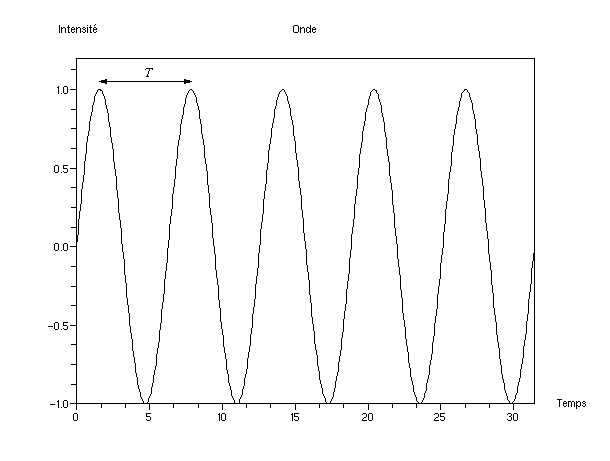
\includegraphics[width=0.8\textwidth]{slide003_2b48e4b2.png}
\end{figure}

Not all waves travel…

…at a fixed point in space

\begin{figure}[H]
\centering
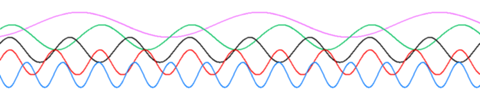
\includegraphics[width=0.8\textwidth]{slide003_3057ad1b.png}
\end{figure}

\begin{figure}[H]
\centering
\includegraphics[width=0.8\textwidth]{slide003_3fdced3d.gif}
\end{figure}

standing waves

\section{Frequency and wavelength}

l

l/T = lf = v

\section{Light}

particles

or

Waves

?

+

reflection, refraction

shadows

Electromagnetic and quantum theory are in perfect agreement if we assume that the amplitude of a field (electric or magnetic) at a certain point and at a certain instant is proportional to the probability (wave function) of finding a photon

\begin{figure}[H]
\centering
\includegraphics[width=0.8\textwidth]{slide005_87b51c96.gif}
\end{figure}

\begin{figure}[H]
\centering
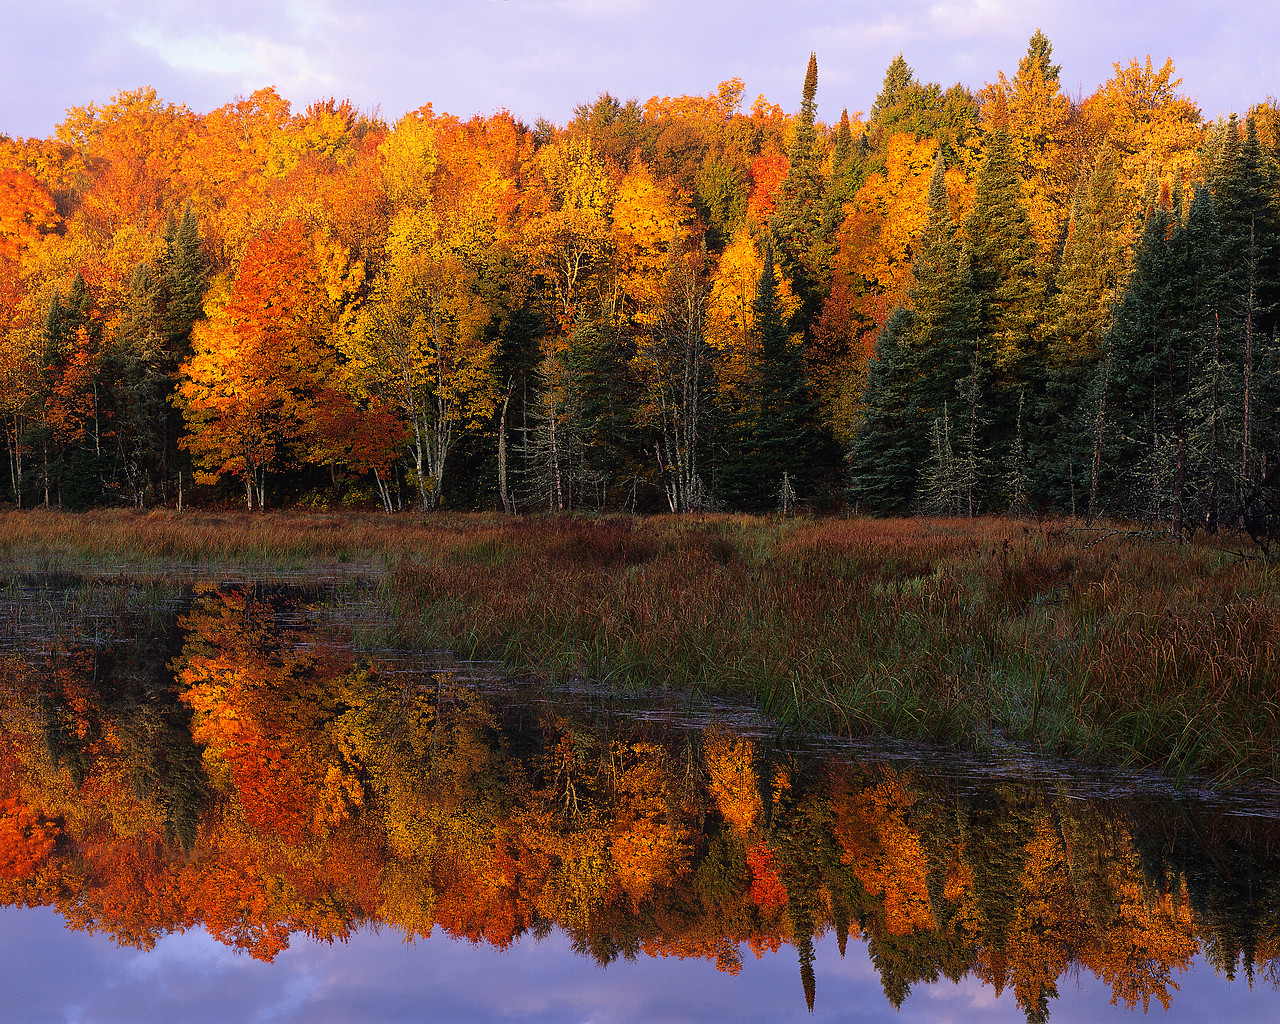
\includegraphics[width=0.8\textwidth]{slide005_77763c66.jpg}
\end{figure}

\begin{figure}[H]
\centering
\includegraphics[width=0.8\textwidth]{slide005_8863b783.gif}
\end{figure}

\begin{figure}[H]
\centering
\includegraphics[width=0.8\textwidth]{slide005_d2480124.gif}
\end{figure}

\section{Light properties}

Reflection

qr

qi

\begin{figure}[H]
\centering
\includegraphics[width=0.8\textwidth]{slide006_e85e96fc.wmf}
\end{figure}

qi = qr

n1

n2

qt

n1sinqi = n2sinqt

Refraction

\section{Refractive indices}

\begin{figure}[H]
\centering

\includegraphics[width=0.8\textwidth]{slide007_24462c13.jpg}
\end{figure}

\section{Why refraction?}

\begin{figure}[H]
\centering
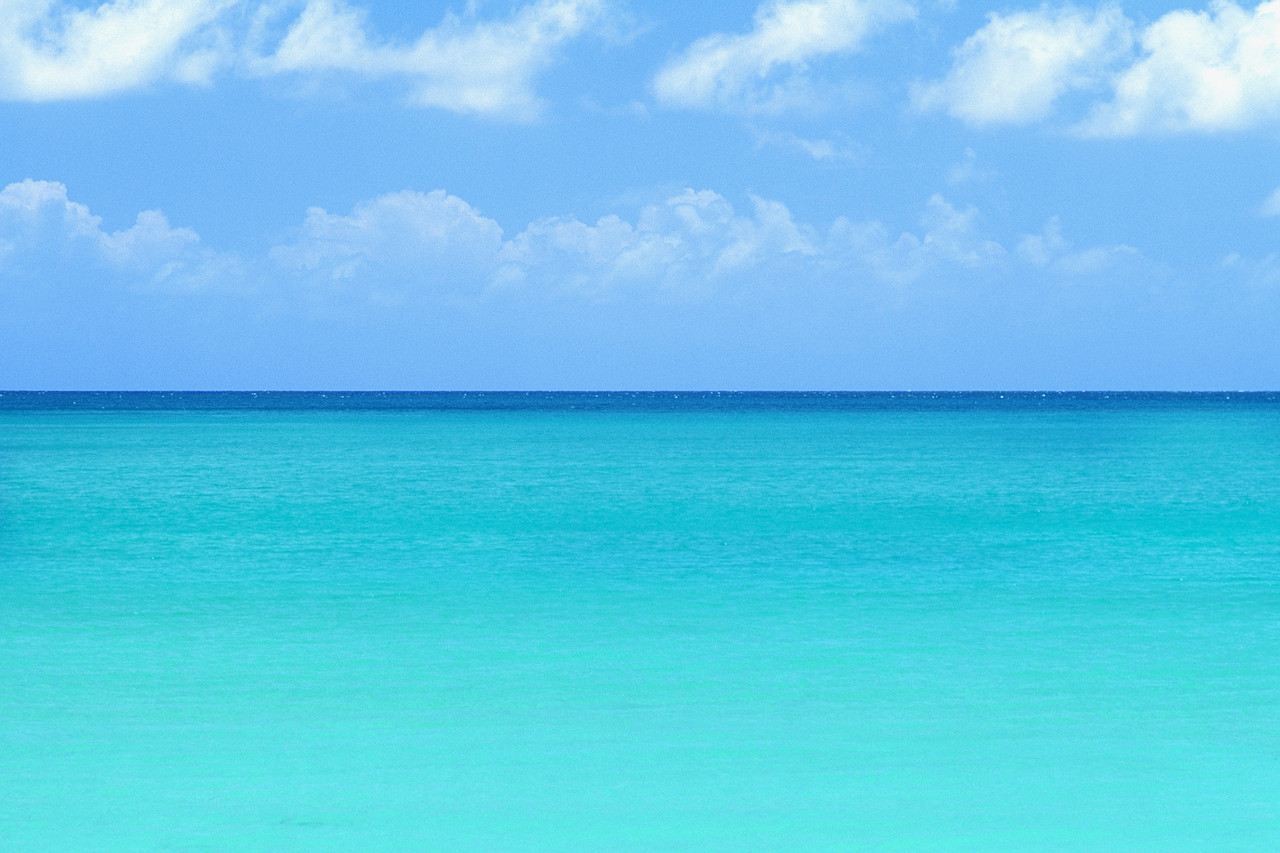
\includegraphics[width=0.8\textwidth]{slide008_0a658c35.jpg}
\end{figure}

n1 = 1

\begin{figure}[H]
\centering

\includegraphics[width=0.8\textwidth]{slide008_61aac317.png}
\end{figure}

?

n2 = 1,3

\section{Interference: some pretty simple math...}

\begin{figure}[H]
\centering
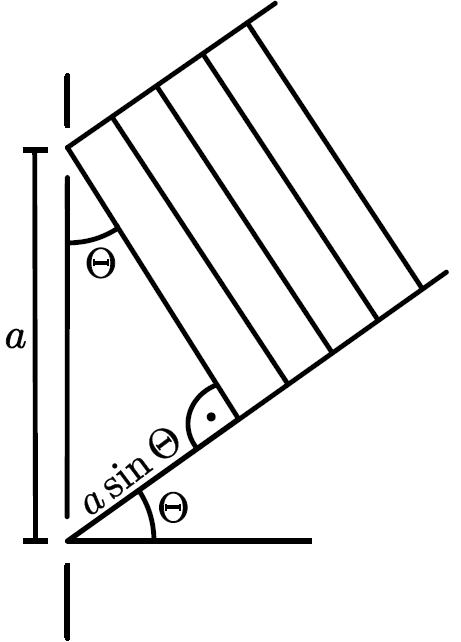
\includegraphics[width=0.8\textwidth]{slide009_250ad787.png}
\end{figure}

\begin{figure}[H]
\centering
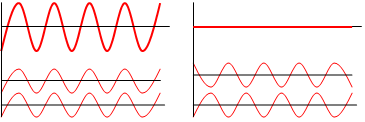
\includegraphics[width=0.8\textwidth]{slide009_944f3aaa.png}
\end{figure}

asin = n

asin = (n+1/2)

\section{Slide 10}

\begin{figure}[H]
\centering
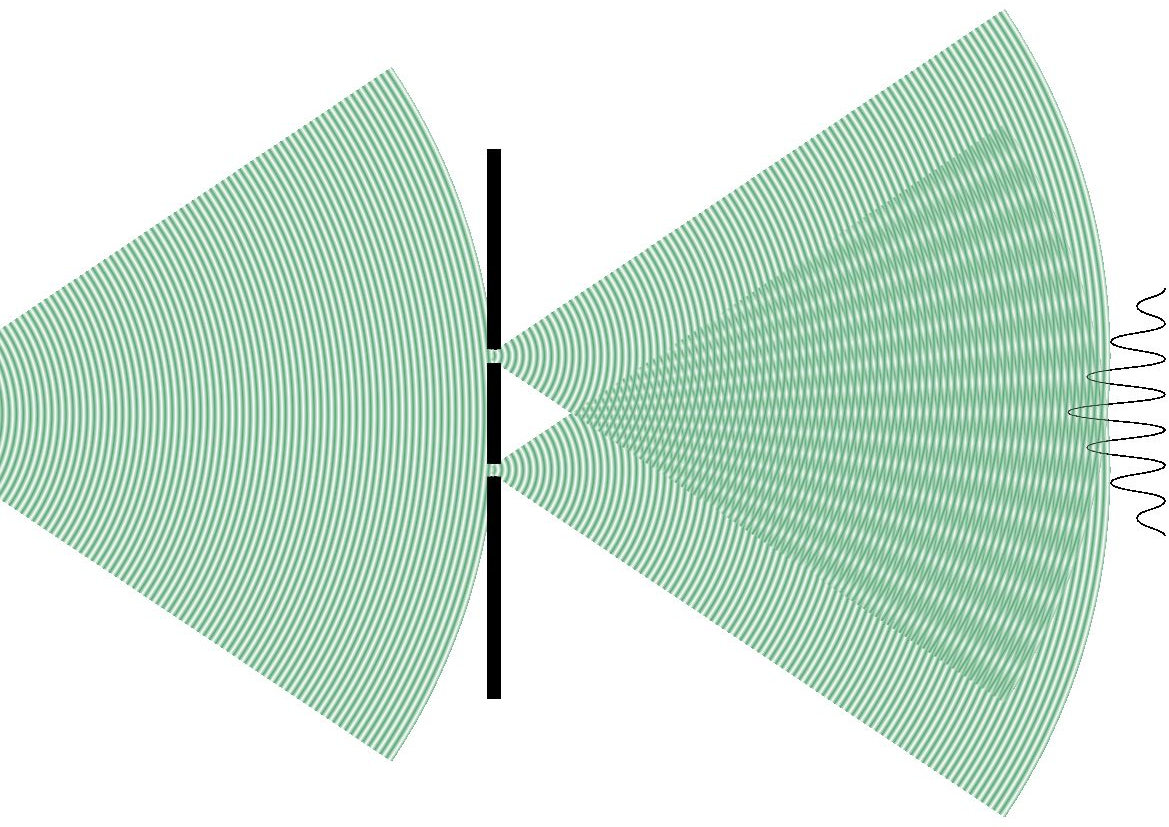
\includegraphics[width=0.8\textwidth]{slide010_a2fbb739.png}
\end{figure}

\begin{figure}[H]
\centering

\includegraphics[width=0.8\textwidth]{slide010_41249af0.png}
\end{figure}

\begin{figure}[H]
\centering
\includegraphics[width=0.8\textwidth]{slide010_310598c7.wmf}
\end{figure}

ngsir.netfirms.com

Web project:

\section{Photoelectric effect}

% Formula da immagine (pix2tex):
\begin{equation}
\begin{array}{c c}{{\displaystyle{\mathcal{L}_{7}\mathcal{L}_{\mathrm{V}}}}}&{{\displaystyle{\begin{array}{c}{{\displaystyle{\ominus}}}\\ {{\displaystyle{\mathcal{L}_{\oplus}^{\qquad}}}}\end{array}\displaystyle{\sqrt{\displaystyle{\Phi_{\mathrm{i}}^{\qquad}}}}}}\\ {{\displaystyle{\left[\stackrel{\ominus\ominus\ominus\ominus\ominus\ominus\ominus\ominus\ominus\ominus\ominus\ominus\ominus\ominus\Phi}{\displaystyle{\oplus\Phi\right]}}}}}\end{array}
\end{equation}

both velocity and energy of electrons independent of light intensity

both velocity and energy of electrons dependent on color of light

electrons insensitive to some colors

\section{Photons}

photons

Light = “energy packets”

E = hf = hc/l   (Planck-Einstein relation)

\begin{figure}[H]
\centering
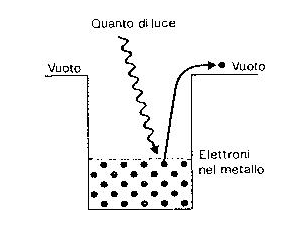
\includegraphics[width=0.8\textwidth]{slide012_eec5fc70.png}
\end{figure}

\section{Electromagnetic spectrum}

\begin{figure}[H]
\centering
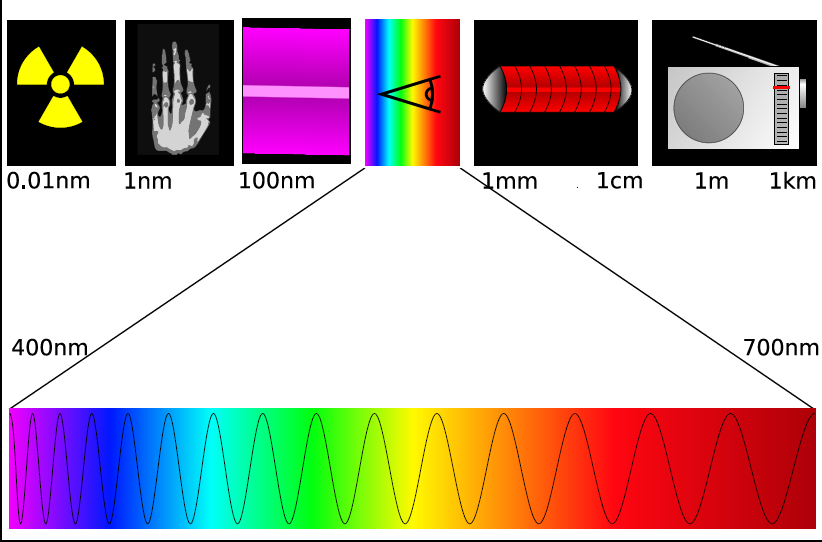
\includegraphics[width=0.8\textwidth]{slide013_93ed602f.png}
\end{figure}

\begin{figure}[H]
\centering
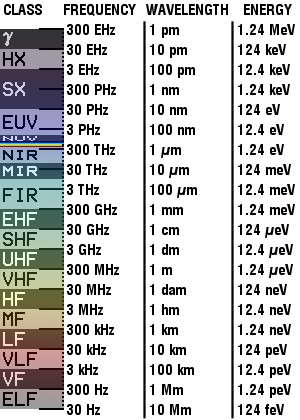
\includegraphics[width=0.8\textwidth]{slide013_f9a25343.png}
\end{figure}

\begin{figure}[H]
\centering
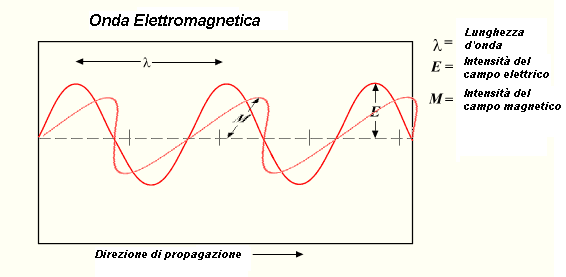
\includegraphics[width=0.8\textwidth]{slide013_ee39dcd4.png}
\end{figure}

\section{Dispersion}

\begin{figure}[H]
\centering
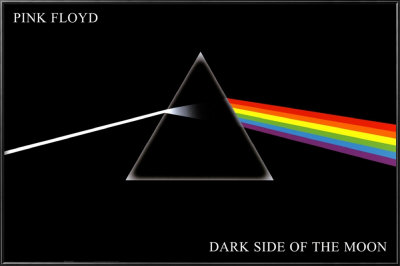
\includegraphics[width=0.8\textwidth]{slide014_53f1e6b2.jpg}
\end{figure}

\begin{figure}[H]
\centering
\includegraphics[width=0.8\textwidth]{slide014_daf17bbb.gif}
\end{figure}

\begin{figure}[H]
\centering
\includegraphics[width=0.8\textwidth]{slide014_e85e96fc.wmf}
\end{figure}

v  function of l

n = n (l)

\begin{figure}[H]
\centering
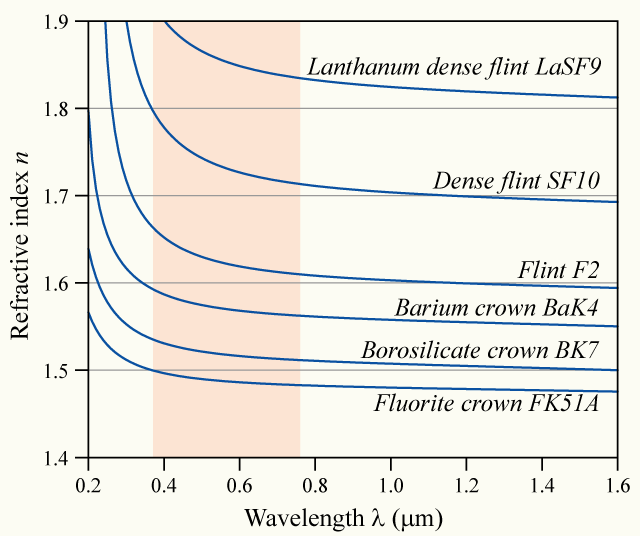
\includegraphics[width=0.8\textwidth]{slide014_13ba3ba0.png}
\end{figure}

\section{Gratings}

\begin{figure}[H]
\centering
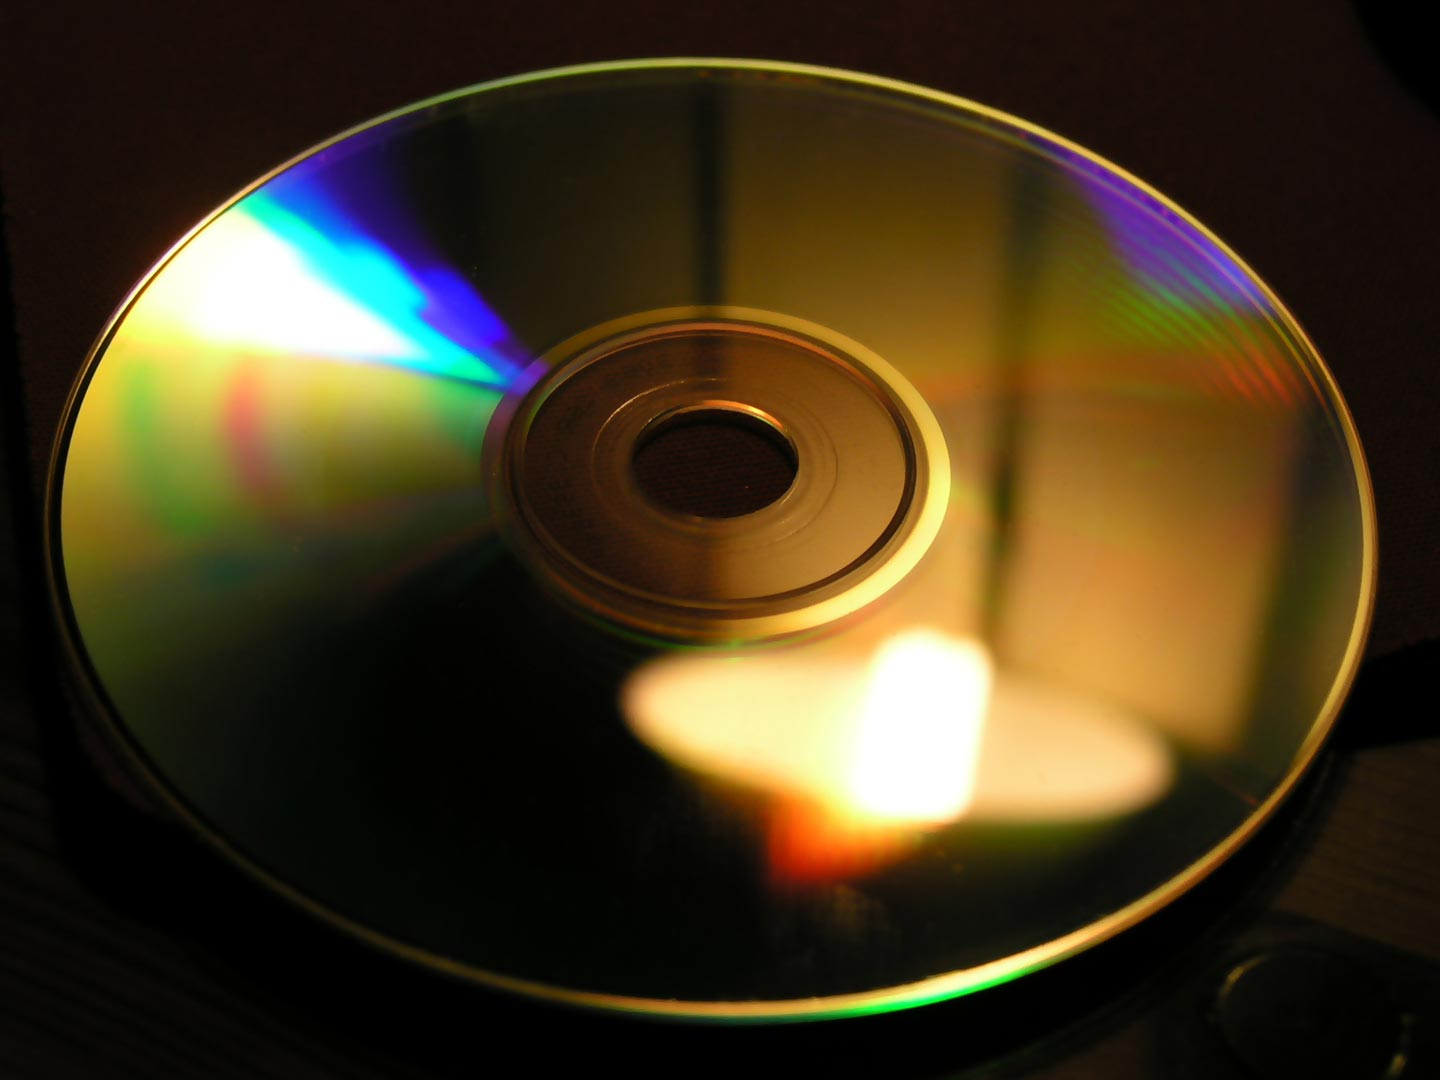
\includegraphics[width=0.8\textwidth]{slide015_147d141d.jpg}
\end{figure}

in reflection

in trasmission

\begin{figure}[H]
\centering
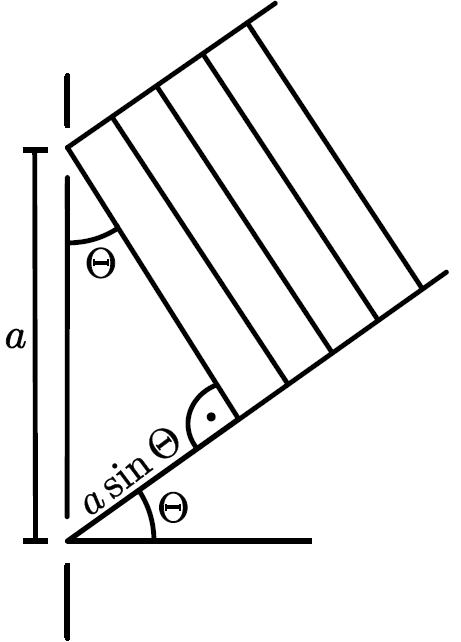
\includegraphics[width=0.8\textwidth]{slide015_250ad787.png}
\end{figure}

\begin{figure}[H]
\centering
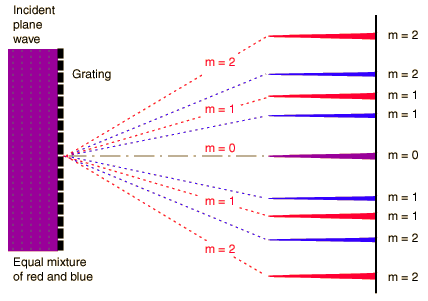
\includegraphics[width=0.8\textwidth]{slide015_dd37f00f.png}
\end{figure}

\begin{figure}[H]
\centering
\includegraphics[width=0.8\textwidth]{slide015_a6274ef4.wmf}
\end{figure}

asin = n

\section{Spectrometer}

\begin{figure}[H]
\centering
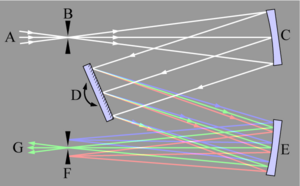
\includegraphics[width=0.8\textwidth]{slide016_dc0eaa88.png}
\end{figure}

\begin{figure}[H]
\centering
\includegraphics[width=0.8\textwidth]{slide016_c7416999.gif}
\end{figure}

mirrors

\begin{figure}[H]
\centering
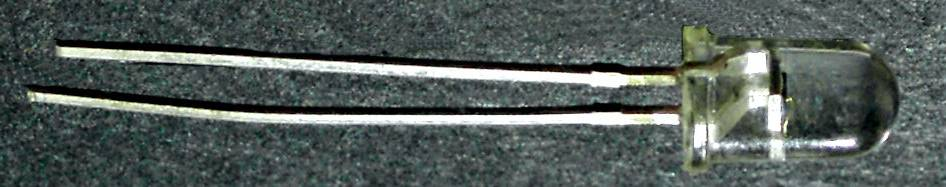
\includegraphics[width=0.8\textwidth]{slide016_66ec243c.jpg}
\end{figure}

slit

resolution?…

\section{Polarization of light}

E

polarized light

H

non-polarized
light

\section{Polarizers}

E

\begin{figure}[H]
\centering
\includegraphics[width=0.8\textwidth]{slide018_310598c7.wmf}
\end{figure}

\section{Optical activity}

ability of some crystals to rotate the wave
polarization plane

possible in crystals that exhibit
birefringence

\section{Light modulation}

\begin{figure}[H]
\centering
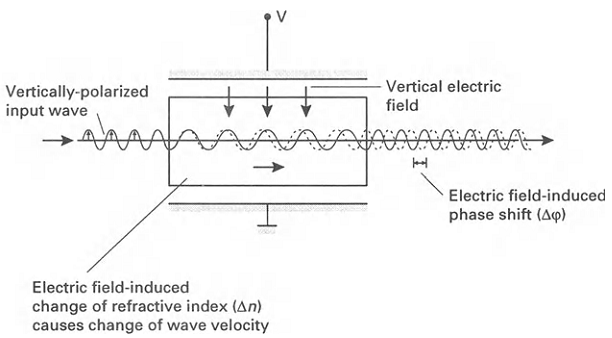
\includegraphics[width=0.8\textwidth]{slide020_836c9c46.png}
\end{figure}

\begin{figure}[H]
\centering
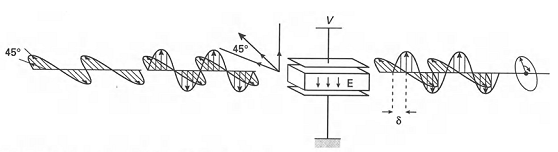
\includegraphics[width=0.8\textwidth]{slide020_39cf8b4c.png}
\end{figure}

% Formula da immagine (pix2tex):
\begin{equation}
\Delta\varphi={\frac{2\pi}{\lambda}}\Delta n\,l
\end{equation}

% Formula da immagine (pix2tex):
\begin{equation}
\mathsf{P o c k e l s~e f f e c t}
\end{equation}

% Formula da immagine (pix2tex):
\begin{equation}
\Delta n=P E
\end{equation}

% Formula da immagine (pix2tex):
\begin{equation}
\Delta n=K E^{2}
\end{equation}

% Formula da immagine (pix2tex):
\begin{equation}
\mathrm{Kerr~effect}
\end{equation}

\section{Light modulation: amplitude modulation}

Light modulation: amplitude modulation

\begin{figure}[H]
\centering
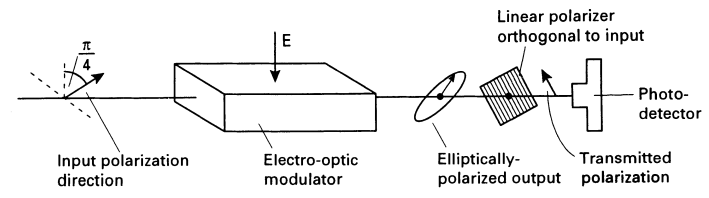
\includegraphics[width=0.8\textwidth]{slide021_d3979c9b.png}
\end{figure}

= f(t)


\end{document}
